\documentclass[11pt]{article}
\usepackage[margin=0.7in, top=0.5in]{geometry}
\usepackage[all]{nowidow}
\usepackage[hyperfigures=true, hidelinks, pdfhighlight=/N]{hyperref}
\usepackage[separate-uncertainty=true, group-digits=false]{siunitx}
\usepackage{graphicx,amsmath,physics,tabto,float,amssymb,pgfplots,verbatim,tcolorbox}
\usepackage{listings,xcolor,caption,import,wrapfig,biblatex,subcaption,pdfpages}
\usepackage[version=4]{mhchem}
\usepackage[noabbrev]{cleveref}
\newcommand{\creflastconjunction}{, and\nobreakspace}
\newcommand{\mb}[1]{\mathbf{#1}}
\newcommand{\chisq}{\chi^2}
\newcommand{\chisqdof}{\chi^2/\mathrm{dof}}
\numberwithin{equation}{section}
\numberwithin{figure}{section}
\numberwithin{table}{section}
\definecolor{stringcolor}{HTML}{C792EA}
\definecolor{codeblue}{HTML}{2162DB}
\definecolor{commentcolor}{HTML}{4A6E46}
\captionsetup{font=small, belowskip=0pt}
\lstdefinestyle{appendix}{
    basicstyle=\ttfamily\footnotesize,commentstyle=\color{commentcolor},keywordstyle=\color{codeblue},
    stringstyle=\color{stringcolor},showstringspaces=false,numbers=left,upquote=true,captionpos=t,
    abovecaptionskip=12pt,belowcaptionskip=12pt,language=Python,breaklines=true,frame=single}
\lstdefinestyle{inline}{
    basicstyle=\ttfamily\footnotesize,commentstyle=\color{commentcolor},keywordstyle=\color{codeblue},
    stringstyle=\color{stringcolor},showstringspaces=false,numbers=left,upquote=true,frame=tb,
    captionpos=b,language=Python}
\renewcommand{\lstlistingname}{Appendix}
\pgfplotsset{compat=1.17}
\addbibresource{bibliography.bib}

\begin{document}

\begin{center}
    {\huge How Much Higgs?}\\
    \vspace{0.2in}
    \textbf{KDSMIL001 | September 2022}
    
    
\end{center}

\section{Introduction}\label{sec:Introduction}
This report aims to investigate the $\chi^2$ and p-value test statistics using data from the ATLAS experiment, reconstructing the mass of the Higgs boson from the 4-lepton system. Our model gives us predictions for the background signal as well as the signal coming from the Higgs. To fit this model to our data we had two parameters to choose from: $s_s$ multiplying the Higgs signal and $s_b$ multiplying the background. 

We first attempted fitting our model with just one parameter at a time, finding the $\chisqdof$ value for each fit. We could then try fitting with both parameters at the same time and look at that $\chisqdof$ value, comparing it to the one-parameter fits. 

The p-value for the model before and after the fitting was the next thing in our sights, comparing the two to decide how likely the it is that the fitted model correctly describes the data we see. 

Lastly we investigated the critical value needed to construct a confidence interval of $68\%$ for a two-parameter fit

\section{Exercises}\label{sec:Exercises}
\subsection{Before fitting}
Before fitting our model to the data, we first looked at the quality of the fit as it came from the data provided. \Cref{fig:no_fit_hist} shows the data, with $\chisqdof=\num{1.598}$. This is a reasonable value as it's close to 1, but we can definitely do better. Note that for this report the $\chisqdof$ values will be approximate, rounding to 3 decimal places. This was chosen as any precision past 3 decimal places seemed to be insignificant in relation to the differences in $\chisqdof$ between fits.

\begin{figure}[h]
    \begin{center}
        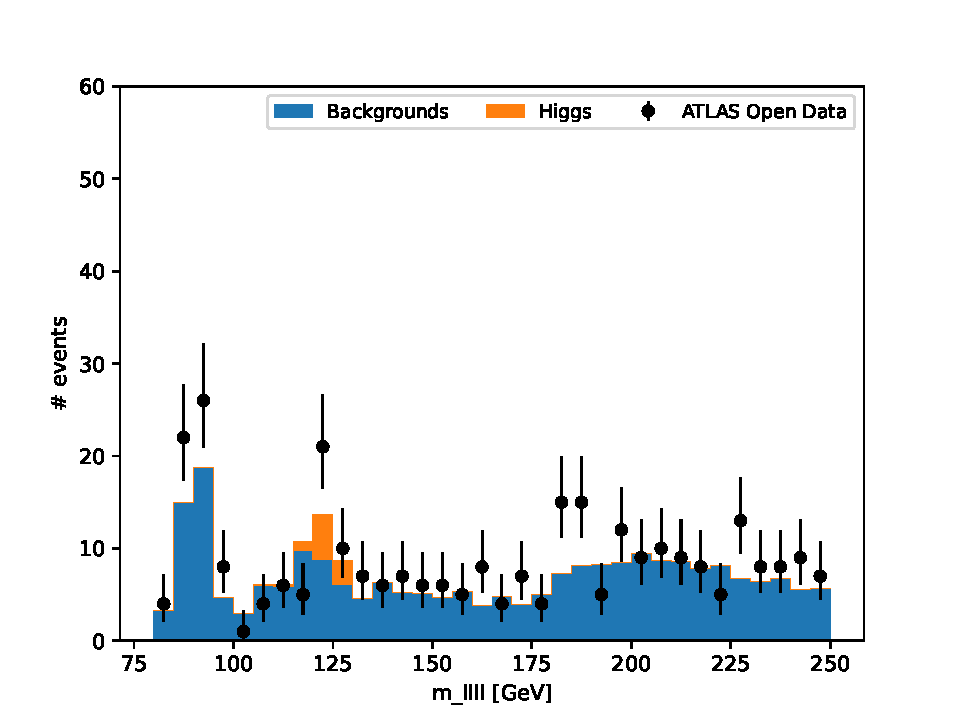
\includegraphics[width=.6\textwidth]{Plots/no_fit_hist.pdf}
        \caption{ATLAS open data of the mass of the 4-lepton system around the predicted mass of the Higgs boson. Also shown is the simulated prediction for the distribution of masses, made up of a background signal and a Higgs signal. For this model, $\chisqdof=\num{1.598}$.}
        \label{fig:no_fit_hist}
    \end{center}
\end{figure}

\subsection{One-parameter fits}
Our first attempts at fitting the model to our data were one-parameter fits, changing the multiplicative factor $s_s$ for the Higgs signal first. At each new value we found a $\chisq$ value for the fit then subtracted the lowest value from the entire set, giving us a $\Delta\chisq$ value for each $s_s$ value in our interval. For a one-parameter fit, a confidence interval of $68\%$ is defined as all values for which $\Delta\chisq\leq1$~\cite{XRay_energy_spectra}. From this we could extract an uncertainty on the best-fit parameter. Our best-fit value was found to be $s_s=\num{2.01 \pm0.76}$ with $\chisqdof=1.558$.

Doing the same but for $s_b$, multiplying the background signal, we found $s_b=\num{1.302\pm0.076}$ with $\chisqdof=1.018$. This parameter clearly has more of an impact on the fit than $s_s$ as can be seen from the lower $\chisqdof$ value. It also has a smaller uncertainty, which we can take as an indication that $s_b$ is the right parameter to vary as our algorithm is quite sure that it should be around 1.3, not just 1.

\subsection{A two-parameter fit}\label{sec:twoParamFit}
Of course, fitting just one parameter at a time is naive, so we then fit them both at the same time, looping over both and finding the minimum $\chisq$ point. This gave us best-fit values of $s_s=1.39^{+1.16}_{-0.87}$ and $s_b=1.29^{+0.12}_{-0.11}$ with $\chisqdof=1.039$. The estimation of these uncertainties came again from the $68\%$ confidence interval, defined for a two-parameter fit as all pairs of values for which $\Delta\chisq\leq2.3$~\cite{XRay_energy_spectra}. \Cref{fig:two_fit_contour} shows the contour plot of $\Delta\chisq$ with respect to the $(s_s,\,s_b)$ pair as well as the contour of the critical value 2.3 defining the confidence interval. Fixing one parameter at its best-fit value, we were able to extract the upper and lower bound on the uncertainty for each parameter. This critical value of 2.3 will be investigated later on. \Cref{fig:two_fit_hist} shows the model fit to the data.


\begin{figure}[h]%
    \centering
    \begin{subfigure}{.5\textwidth}
        \centering
        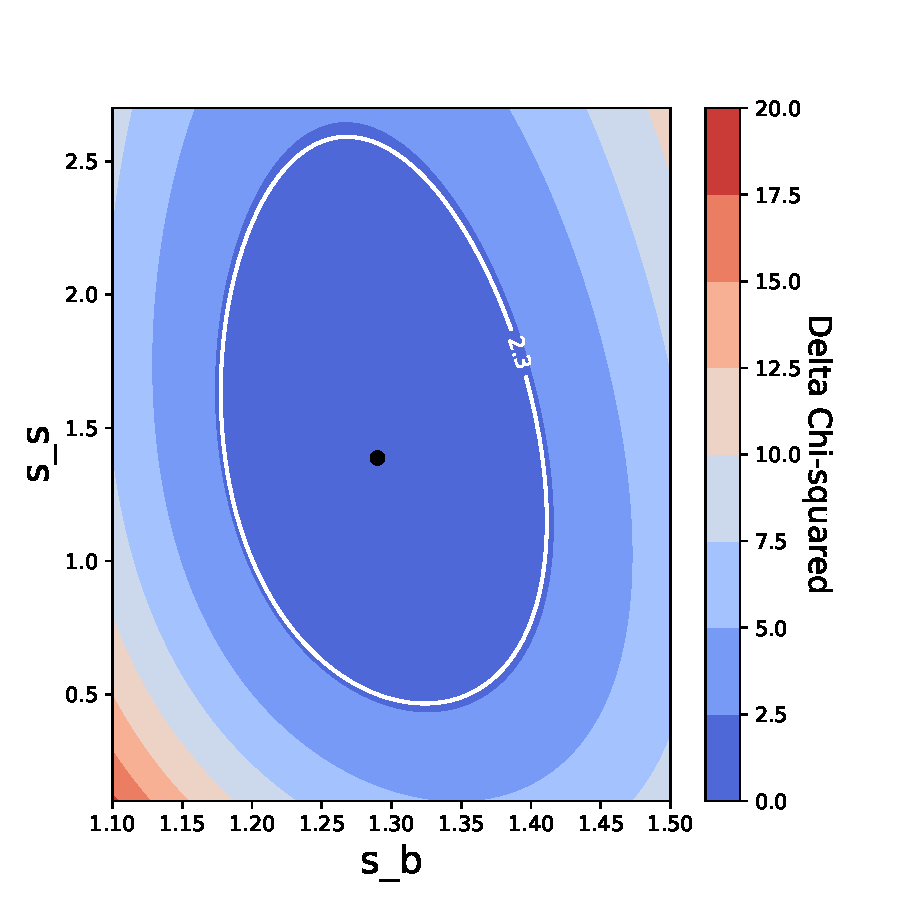
\includegraphics[width=0.98\linewidth]{Plots/two_fit_contour.pdf}
        \caption{Contour plot showing the $\Delta\chisq$ value for each $(s_s,\,s_b)$ pair. The confidence interval on the best-fit pair (black dot) is shown as the area inside the contour at $\Delta\chisq=2.3$. Upper and lower bounds on the confidence interval for each parameter were extracted to determine uncertainties.}
        \label{fig:two_fit_contour}
    \end{subfigure}\;%
    \begin{subfigure}{.5\textwidth}
        \centering
        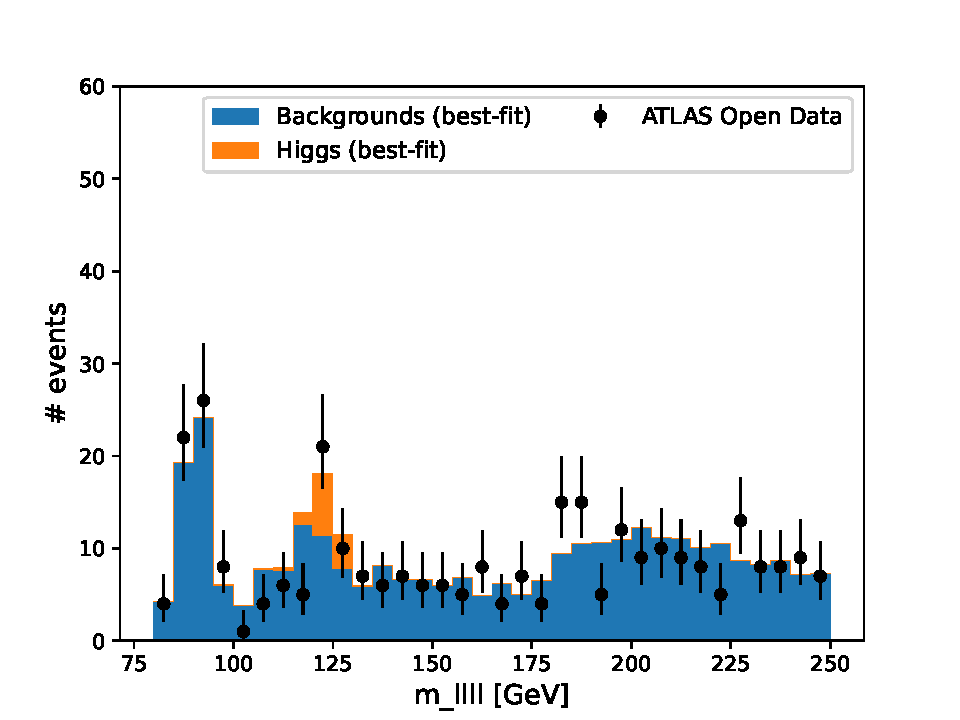
\includegraphics[width=0.98\linewidth]{Plots/two_fit_hist.pdf}
        \caption{Histogram showing the data and the newly fitted model. $s_s=1.39^{+1.16}_{-0.87}$, $s_b=1.29^{+0.12}_{-0.11}$, and $\chisqdof=1.039$.}
        \label{fig:two_fit_hist}
    \end{subfigure}
    \caption{Contour plot and histogram for the two-parameter fit.}
    \label{fig:two_fit}
\end{figure}

\subsection{Comparing the one- and two-parameter fits}
As seen before, the one-parameter fitting was much better when changing the scale of the background signal as opposed to the Higgs signal. This seems to make sense as the background signal is present over the entire range of interest, while the Higgs signal is only significant for a few of the bins in \cref{fig:no_fit_hist}, so we might expect that changing the scale of the background has a larger impact on the overall fit of the model to our data. What is interesting about the two-parameter fit is that its $\chisqdof$ value is actually larger than that for the one-parameter background fit. Not only that, but the uncertainties on both $s_s$ and $s_b$, for their respective one-parameter fits, are smaller than those determined from the two-parameter fit. 

We can compare the best-fit values at a basic level, noting that for the two-parameter fit, $s_s$ is a fair bit smaller than when fit on its own. This makes sense as in the two-parameter fit, the signal has already been lifted by the now larger background signal. It doesn't make sense, however, to compare the values with respect to their uncertainties, saying whether they agree or disagree. The reason for this is exactly what has been said: the signal sits on top of a different background, so it's been shifted by some amount. The fact that the best-fit $s_b$ value doesn't change by much makes sense as well as its goal is to optimise the fit over the entire range of interest, only a small portion of which contains the Higgs signal. For this reason, it's likely to settle on the same best-fit value whether we include $s_s$ or not.

We can also examine the shape of the $\Delta\chisq=2.3$ contour in \cref{fig:two_fit_contour}, noting that it is slightly asymmetric. If it were a perfect ellipse with its axes aligned with the axes of the plot, we would be able to say there is no correlation between $s_s$ and $s_b$, but there is clearly a non-zero amount of negative correlation, as well as an asymmetry as can be seen by the uneven shape at the bottom.

\subsection{Goodness of fit}
The p-value statistic is another useful measure of the goodness of fit of a model to some data. It is closely related to $chisq$ but offers a different interpretation. Before fitting, so for \cref{fig:no_fit_hist}, we found $p=0.014877$. This means that if we assume our model to be correct, the chance of seeing the data we did, or anything more extreme, is around $1.5\%$. In other words, it's not that likely that this model is correct. After our two-parameter fit we found $p=0.40642$, meaning that there's around a $41\%$ chance to see data as or more extreme than ours, given our model is true. This is much better as, if the model perfectly described the process that created the data, we would expect an average p-value of 0.5 over many sets of data. Clearly our fitting process improved our model considerably. 

\subsection{Investigating the critical value for a two-parameter fit}
Earlier, we simply quoted the critical value for a two-parameter fit as being 2.3, supported by Avni~\cite{XRay_energy_spectra}, but we would like to verify for ourselves that this is the correct value. To restate the problem, we need to find the critical value, which we will call $d$, for which $68\%$ of all experiments have the ``true value'' within the region defined by that $d$. The true value in this case is the pair of best-fit values found before. To do this we generate a number of toy datasets, generating random bin values distributed according to gaussian distributions with means equal to the bin values of the fitted model and standard deviations equal to the square root of the means. We then check, for a range of $d$ values, what fraction $f$ of these toys have the best-fit pair within the confidence interval defined by $d$ and the $\Delta\chisq$ array for that toy. \Cref{fig:d_f} shows the results.

\begin{figure}[h]
    \begin{center}
        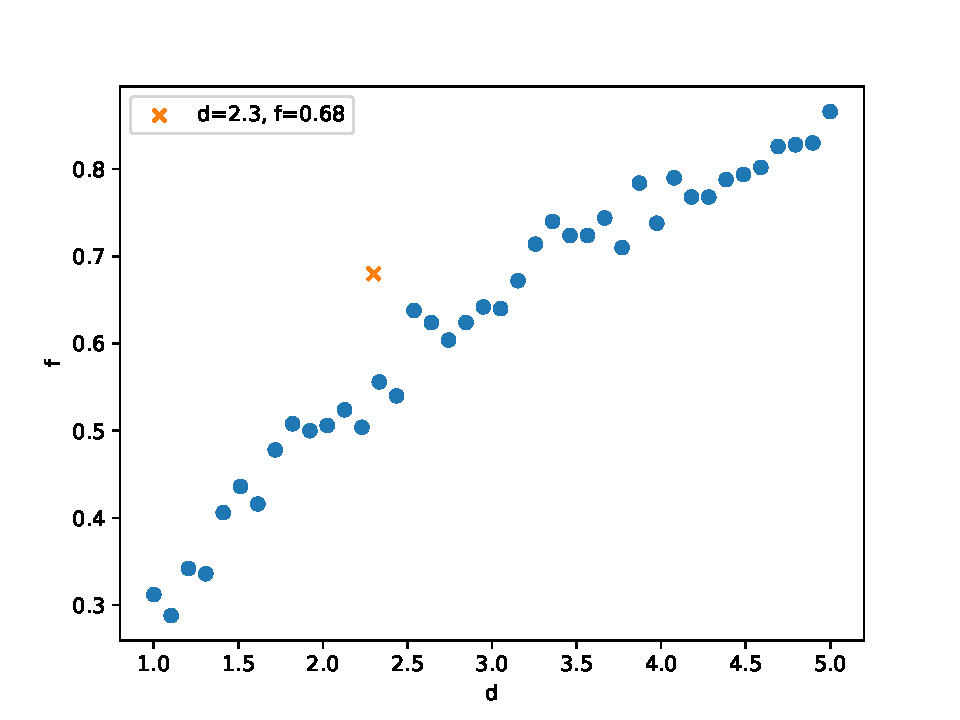
\includegraphics[width=.8\textwidth]{Plots/d_f.pdf}
        \caption{Fraction of toys $f$ whose confidence interval for a given $d$ contains the best-fit point as determined in \cref{sec:twoParamFit}. Shown in orange is the expected $d$ value for a fraction of 0.68 for a two-parameter fit. For each $d$ value, 500 toys were used.}
        \label{fig:d_f}
    \end{center}
\end{figure}

What can easily be seen in \cref{fig:d_f} is that a fraction of 0.68 apparently requires a critical value of around 3.3, quite far off the theoretical value of 2.3. This discrepancy could have a number of explanations. 

Firstly, our search for the best-fit values was never going to return the exact right parameter values as we searched on a grid with a fixed spacing. It's more likely than not that the true value actually lies somewhere between the points that our method could test. Another method, perhaps using a gradient descent method or shrinking the grid spacing a few times to hone in on the value, would have yielded more accurate results. 

Secondly, we made what we believe to be an incorrect assumption about the distribution of bin values. We needed to assume that they were gaussian distributed in order to generate the toys, but given that the best-fit model has bin values around 10 to 20, it's not safe to assume a gaussian distribution as there are just too few events per bin. It is for this reason that we see $f$ trending to a more shallow gradient as $d$ increases and thus our critical value for a $68\%$ confidence interval becomes about 3.3. 

\section{Conclusion}\label{sec:Conclusion}



\newpage
\printbibliography

% \newpage
% \appendix
% \section{Code}
% % \setcounter{figure}{0} \renewcommand{\thefigure}{A.\arabic{figure}}
% 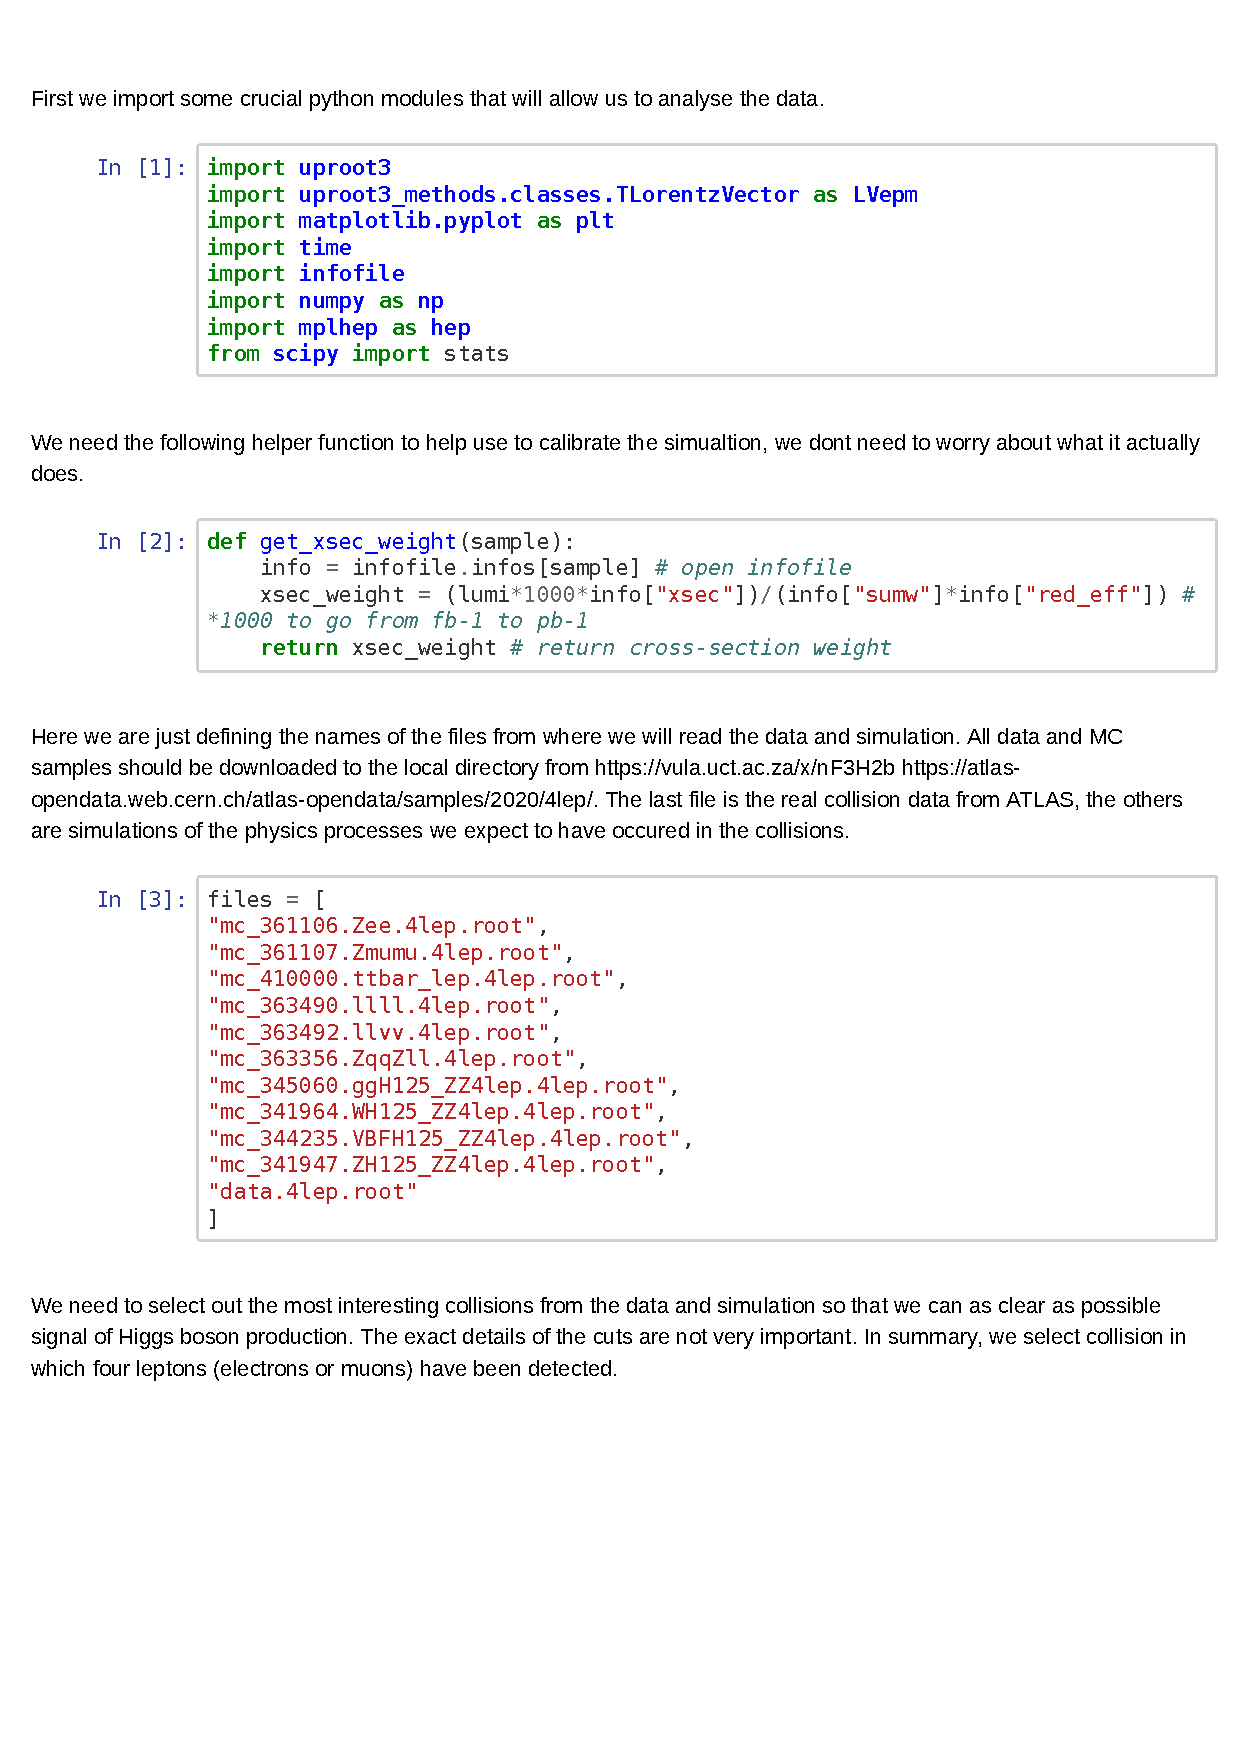
\includepdf[pages=-]{code.pdf}

\end{document}